% algorithmes de flot max

\begin{frame}{Le problème du flot maximal}
    \begin{itemize}
        \item Capacité de transport : réseaux de trains, de canalisation, câbles électriques, réseaux d'information, réseaux routiers, infrastructures de transport multimodales\dots
        \item La question : combien (d'information, d'eau, de touristes, de voitures,  d'élections\dots) peut-on faire transiter sur ce réseau ?
        \item Formalisation : faire passer la plus grande quantité de matière entre une source $s$ et une destination $t$. Les liens permettant d'acheminer le flux ont une \emph{capacité} limitée et il n'y a ni perte ni création de matière lors de l'acheminement 
        \item On se donne 
        \begin{itemize}
            \item un graphe orienté $G=(S,A)$
            \item une capacité $c : A \longrightarrow \nbR^+$
            \item 2 sommets particuliers de $S$ : $s$ et $t$ 
        \end{itemize}
    \end{itemize}
\end{frame}

\begin{frame}{Problème du flot maximal}
    \begin{definition}
        Un \emph{flot} est une fonction $f : A \longrightarrow \nbR^+$ telle que 
        \begin{itemize}
            \item $0 \leq f(a) \leq c(a), \forall a \in A$ (contrainte de capacité)
            \item $ \sum_{(i,j) \in A} f(i,j) = \sum_{(j,k) \in A} f(j,k) \forall j \neq s,t$ (contrainte de conservation)
        \end{itemize}
    \end{definition}
    \begin{itemize}
        \item Pour vérifier la loi de conservation en tous sommets, on va ajouter au graphe un arc de retour fictif entre $t$ et $s$ et on appellera \emph{valeur du flot} $val(f)$ la quantité $f(t,s)$ 
        \item On cherche alors à maximiser $val(f)$ 
        \item NB : c'est un programme linéaire sous contraintes !
    \end{itemize}
\end{frame}

\begin{frame}{Représentation graphique}
    \begin{center}
        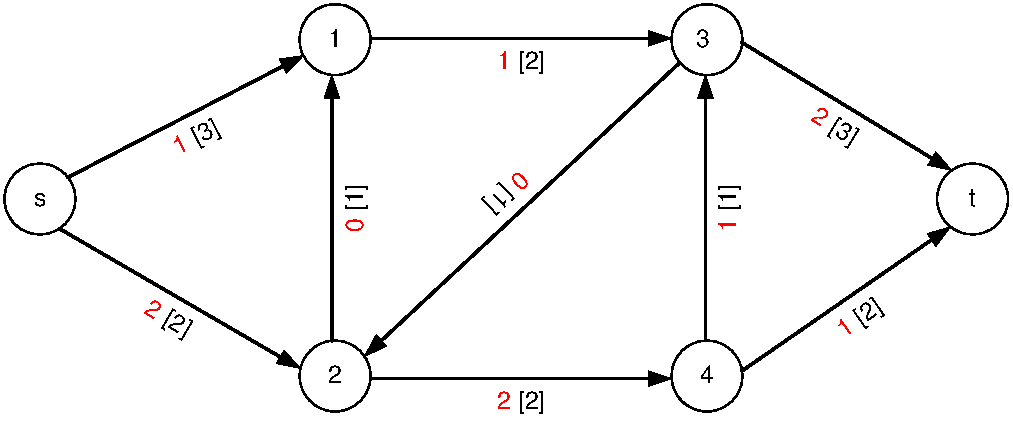
\includegraphics[height=.5\textheight]{fig/flot1.pdf}
    \end{center}
    Convention : la capacité est représentée entre crochets 
\end{frame}

\begin{frame}{Représentation graphique avec arc de retour fictif}
    \begin{center}
        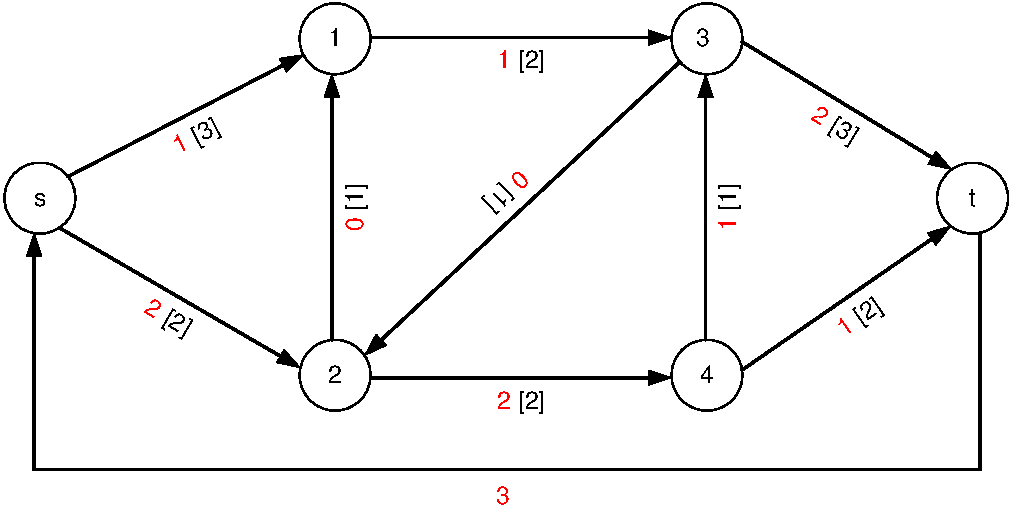
\includegraphics[height=.5\textheight]{fig/flot2.pdf}
    \end{center}
\end{frame}

\begin{frame}{Algorithme de Ford-Fulkerson}
    \begin{itemize}
        \item Principe 
        \begin{itemize}
            \item Le flot nul est toujours réalisable : point de départ
            \item Idée : si on trouve d'un chemin d'arcs non saturés de $s$ à $t$, alors on peut augmenter le flot le long de ce chemin 
        \end{itemize}
        \item pour un flot donné, capacité résiduelle d'un arc $a$ : $c^r(a) = c(a) - f(a)$
        \item on dit qu'un arc est saturé si sa capacité résiduelle est nulle, $c^r(a) = 0$
        \item \textbf{Mais cette notion n'est pas toujours suffisante !}
        \begin{itemize}
            \item en clair, risque de minimum local 
        \end{itemize}
    \end{itemize}
\end{frame}

\begin{frame}{Chaine augmentante}
    \begin{definition}
        Une chaine augmentante de $s$ à $t$ pour un flot admissible donné est une chaine respectant les contraintes suivantes :
        \begin{itemize}
            \item $f(a) < c(a)$ pour tout arc $a$ dirigé de $s$ vers $t$ 
            \item $f(a) > 0$ pour tout arc dirigé de $t$ vers $s$
        \end{itemize}
    \end{definition}    
    \begin{example}
        \begin{center}
            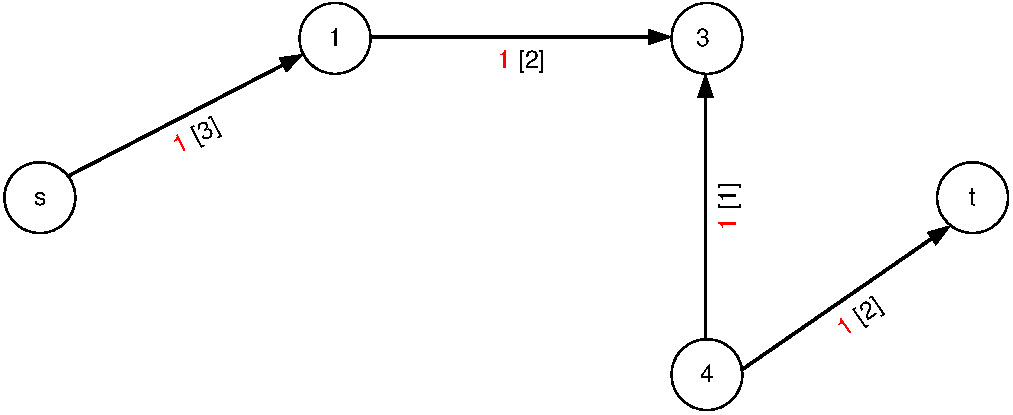
\includegraphics[height=0.35\textheight]{fig/flot3.pdf}
        \end{center}
        
    \end{example}
\end{frame}

\begin{frame}{Augmentation du flot le long d'une chaine augmentante}
    \begin{itemize}
        \item Le flot peut alors être augmentée d'une quantité $\alpha$ définie par 
        $$
        \alpha = \min \left[ 
            min_{a \in \mu^+} (c(a) - f(a)) , \min_{a \in \mu^- } f(a)
        \right]
        $$
        \item où $\mu^+$ (respectivement $\mu^-$) est l'ensemble des arcs orientés de $s$ vers $t$ dans la chaine (respectivement de $t$ vers $s$)
        \item On peut alors augmenter le flot de $\alpha$ sur les arcs de  $\mu^+$ et le diminuer de $\alpha$ sur les arcs de $\mu^-$
    \end{itemize}
\end{frame}

\begin{frame}{Coupes}
    \begin{definition}
        Une st-coupe associée à un graphe $G=(X,A)$ est une partition de $X$ en deux ensembles $S$ et $T$ tels que $s \in S$ et $t \in T$. 
        
        On appelle capacité de cette st-coupe $c(S,T) = \sum_{i \in S, j \in T} c(i,j)$ 
    \end{definition}
    \begin{theorem}
        Un flot de $s$ à $t$ est maximal s'il n'existe pas de chaine augmentante de $s$ à $t$.
    \end{theorem}
    \begin{block}{Corollaire}
        Quelle que soit la st-coupe $(S,T)$, quel que soit le flot $f$, la valeur du flot $val(f)$ est inférieure ou égale à la capacité de cette coupe : $val(f) \leq c(S,T)$.
    \end{block}
\end{frame}

\begin{frame}{Théorème de Ford-Fulkerson}
    \begin{theorem}
        La valeur du flot maximal est égal à la capacité de la coupe minimale 
    \end{theorem}
\end{frame}

\begin{frame}{Schéma de l'algorithme de Ford-Fulkerson}
    \begin{algorithmic}
        \Function{ff}{(G,s)}
        \State x = (0,...,0) 
        \While{il existe une chaine augmentante de $s$ à $t$} 
            \State $c$ \gets chaine augmentante de $s$ à $t$
            \State $\mu^+$ \gets arcs de $c$ dans le sens $s$ vers $t$ 
            \State $\mu^-$ \gets arcs de $c$ dans le sens $t$ vers $s$
            \State $\alpha = \min \left[ 
                min_{a \in \mu^+} (c(a) - f(a)) , \min_{a \in \mu^- } f(a)
            \right]$
            \For{$a \in \mu^+$} 
                $f(a)$ \gets $f(a)+\alpha$
            \EndFor
            \For{$a \in \mu^-$} 
                $f(a)$ \gets $f(a)-\alpha$
            \EndFor
        \EndWhile
        \EndFunction
    \end{algorithmic}
\end{frame}

\begin{frame}{Déterminer une chaine augmentante}
    \begin{itemize}
        \item Un point n'est pas abordé dans l'algorithme précédent : comment déterminer une chaine augmentante ?
    \end{itemize}
    \begin{definition}
        On appelle \emph{graphe résiduel} $G^r=(S,A^r)$ le graphe associé à une capacité et à un flot donné, avec $\forall a \in A$ :
        \begin{itemize}
            \item si $f(a) < c(a)$ alors on ajoute $a$  $A^R$ avec $c^r(a) = c(a)-f(a)$
            \item si $f(a) > 0$ alors on ajoute $a$ \textbf{en sens inverse} dans $A^r$ avec une capacité égale à $f(a)$
        \end{itemize}
    \end{definition}
\end{frame}


\begin{frame}{Graphe résiduel : exemple}
\begin{center}
    \scalebox{0.65}{\begin{tikzpicture}
\clip (0,0) rectangle (9.0,6.0);
\Vertex[x=0.450,y=3.000,size=0.5,opacity=0.5,label=s]{0}
\Vertex[x=3.150,y=5.700,size=0.5,opacity=0.5,label=A]{1}
\Vertex[x=3.150,y=1.920,size=0.5,opacity=0.5,label=B]{2}
\Vertex[x=3.150,y=0.300,size=0.5,opacity=0.5,label=C]{3}
\Vertex[x=5.850,y=5.700,size=0.5,opacity=0.5,label=D]{4}
\Vertex[x=6.525,y=3.000,size=0.5,opacity=0.5,label=E]{5}
\Vertex[x=5.850,y=0.300,size=0.5,opacity=0.5,label=F]{6}
\Vertex[x=8.550,y=3.000,size=0.5,opacity=0.5,label=t]{7}
\Edge[,lw=1.0,bend=-12.68,label=20 [35],Direct](0)(1)
\Edge[,lw=1.0,bend=-12.68,label=0 [35],Direct](0)(2)
\Edge[,lw=1.0,bend=-12.68,label=0 [40],Direct](0)(3)
\Edge[,lw=1.0,bend=-12.68,label=20 [20],Direct](1)(4)
\Edge[,lw=1.0,bend=-12.68,label=0 [10],Direct](1)(6)
\Edge[,lw=1.0,bend=-12.68,label=0 [15],Direct](2)(4)
\Edge[,lw=1.0,bend=-12.68,label=0 [25],Direct](2)(5)
\Edge[,lw=1.0,bend=-12.68,label=0 [5],Direct](2)(6)
\Edge[,lw=1.0,bend=-12.68,label=0 [20],Direct](3)(5)
\Edge[,lw=1.0,bend=-12.68,label=0 [20],Direct](3)(6)
\Edge[,lw=1.0,bend=-12.68,label=20 [20],Direct](4)(7)
\Edge[,lw=1.0,bend=-12.68,label=0 [30],Direct](5)(7)
\Edge[,lw=1.0,bend=-12.68,label=0 [60],Direct](6)(7)
\end{tikzpicture}
} 
    \scalebox{0.65}{\begin{tikzpicture}
\clip (0,0) rectangle (9.0,6.0);
\Vertex[x=0.450,y=3.000,size=0.5,opacity=0.5,label=s]{0}
\Vertex[x=3.150,y=5.700,size=0.5,opacity=0.5,label=A]{1}
\Vertex[x=3.150,y=1.920,size=0.5,opacity=0.5,label=B]{2}
\Vertex[x=3.150,y=0.300,size=0.5,opacity=0.5,label=C]{3}
\Vertex[x=5.850,y=5.700,size=0.5,opacity=0.5,label=D]{4}
\Vertex[x=6.525,y=3.000,size=0.5,opacity=0.5,label=E]{5}
\Vertex[x=5.850,y=0.300,size=0.5,opacity=0.5,label=F]{6}
\Vertex[x=8.550,y=3.000,size=0.5,opacity=0.5,label=t]{7}
\Edge[fontcolor=green,lw=1.0,bend=-12.68,label=[20],Direct](1)(0)
\Edge[fontcolor=red,lw=1.0,bend=-12.68,label=[15],Direct](0)(1)
\Edge[,lw=1.0,bend=-12.68,label=[35],Direct](0)(2)
\Edge[,lw=1.0,bend=-12.68,label=[40],Direct](0)(3)
\Edge[fontcolor=green,lw=1.0,bend=-12.68,label=[20],Direct](4)(1)
\Edge[,lw=1.0,bend=-12.68,label=[10],Direct](1)(6)
\Edge[,lw=1.0,bend=-12.68,label=[15],Direct](2)(4)
\Edge[,lw=1.0,bend=-12.68,label=[25],Direct](2)(5)
\Edge[,lw=1.0,bend=-12.68,label=[5],Direct](2)(6)
\Edge[,lw=1.0,bend=-12.68,label=[20],Direct](3)(5)
\Edge[,lw=1.0,bend=-12.68,label=[20],Direct](3)(6)
\Edge[fontcolor=green,lw=1.0,bend=-12.68,label=[20],Direct](7)(4)
\Edge[,lw=1.0,bend=-12.68,label=[30],Direct](5)(7)
\Edge[,lw=1.0,bend=-12.68,label=[60],Direct](6)(7)
\end{tikzpicture}
}
\end{center}
\end{frame} 